
\section{Descrizione del dominio di riferimento e obiettivi della sperimentazione} 

\subsection{Risoluzione di Sistemi Lineari}

Il problema della risoluzione di sistemi lineari attraverso una computazione efficiente è tuttora aperto e al centro di progetti e obiettivi di ricerca.

Allo stato dell'arte attuale si definiscono due tipologie principali di metodologie per la loro risoluzione: i metodi diretti e i metodi iterativi.
I metodi diretti permettono di arrivare ad una soluzione in un numero finito di step e restituirebbero la soluzione esatta sotto l'assunzione di essere eseguiti su un'aritmetica con precisione infinita, cosa in realtà non possibile sui reali calcolatori.

La tecnica di base per una risoluzione di questo tipo è detta \textit{fattorizzazione LU} di una matrice A, che viene scomposta in una \textit{Lower triangular L} e una \textit{Upper triangular U}, con il risultato finale calcolato come segue:

\begin{equation} \label{eq1}
\begin{split}
Ax & = b \\
L(Ux) & = b; Ux = y \\
Ly & = b
\end{split}
\end{equation}

\begin{figure}[h!]
    \centering
    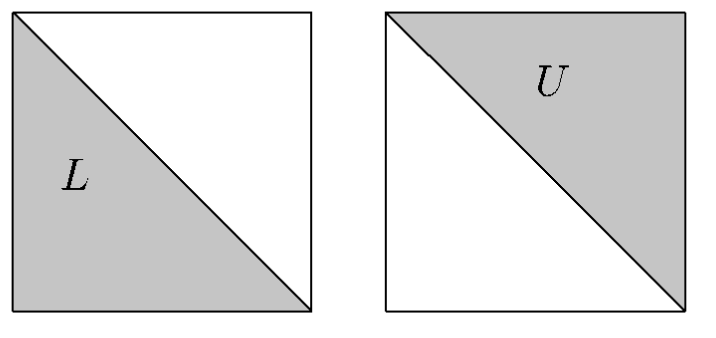
\includegraphics[width=0.5\textwidth]{figs/LU_decomposition.png}
    \caption{LU Decomposition for Direct Methods}
    \label{fig:LU_decomposition}
\end{figure}

Al contrario, i metodi iterativi non assicurano di terminare in un numero finito di step: a partire da un \textit{initial guess} formano iterazioni successive che convergono solo al limite della soluzione esatta. 
Per far sì che l'iterazioni termini, viene utilizzato un criterio di convergenza per specificare quando una soluzione approssima sufficientemente al risultato esatto. 

Anche in caso dell'utilizzo di un'aritmetica con precisione infinita, i metodi iterativi non restituirebbero comunque, in linea teorica, una soluzione esatta, ma il loro vantaggio è quello di essere computazionalmente più efficienti dei diretti, e pertanto più utilizzati nella pratica, sebbene abbiano la necessità di essere eseguiti su matrici che rispettino precise proprietà per essere certi della convergenza. Ad esempio, 2 tra i metodi iterativi più comuni, \textit{Jacobi} e \textit{Gauß-Seidel}, garantiscono la convergenza solo in caso di matrici a dominanza diagonale in input.

Nel presente elaborato viene analizzata la risoluzione di sistemi lineari mediante decomposizione di Cholesky, una particolare tipologia di metodo diretto che sfrutta la proprietà secondo cui, se la matrice \textit{A} è \textit{SDP} (simmetrica e definita positiva), è allora possibile riorganizzare la decomposizione in maniera tale che \textit{U} sia la trasposta di \textit{L}, pertanto \textit{A} possa essere riscritta come

\begin{equation} \label{eq1}
\begin{split}
Ax & = LL'
\end{split}
\end{equation}

\begin{figure}[h!]
    \centering
    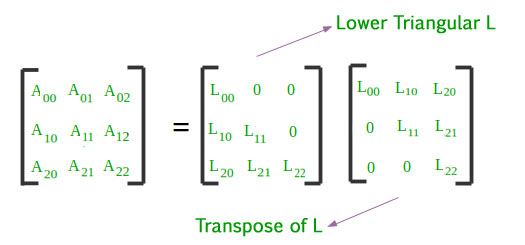
\includegraphics[width=0.75\textwidth]{figs/chol_decomposition.jpg}
    \caption{Basic visualization for Cholesky Decomposition}
    \label{fig:cholesky_decomposition}
\end{figure}

Se la matrice rispetta tale proprietà, allora è garantito che la sua decomposizione di Cholesky esista e sia unica, il che rende la risoluzione del sistema più efficiente e stabile rispetto ad una normale decomposizione \textit{LU}.

Come già visto precedentemente, sebbene si tratti di un metodo di risoluzione diretto, che pertanto dovrebbe, in linea teorica, restituire un risultato esatto a seguito di un numero finito di step, ciò non è garantito dal fatto di utilizzare dei calcolatori non provvisti di precisione aritmetica infinita.
È per questo che tra le analisi presentate in seguito, si terrà conto nella valutazione del miglior risultato, anche dell'errore relativo tra il risultato calcolato e quello atteso, auspicando comunque che esso si avvicini quanto più possibile all'epsilon di macchina, pari a
\[
  2.220446049250313*10^{-16}
\]

\subsection{Matrici Sparse}

Avendo a che fare con dati di dimensioni molto grandi, nelle analisi che seguono sono state utilizzate le matrici sparse: si tratta di matrici con la maggior parte dei valori pari a 0, che vengono memorizzate in maniera compatta, tenendo conto dei soli valori positivi.

\begin{figure}[h!]
    \centering
    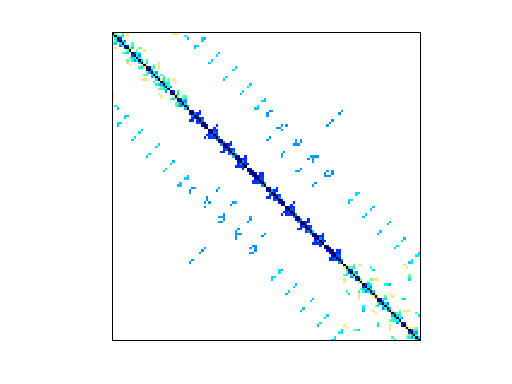
\includegraphics[width=0.5\textwidth]{figs/shallow_water1.png}
    \caption{Sparse matrix example}
    \label{fig:sparse_matrix_example}
\end{figure}

Questo modo di operare permette, oltre al fatto di risparmiare sapzio in memoria a seguito del cricamento della matrice stessa, anche una risoluzione più efficiente della decomposiiizione di Cholesky stessa.

La semplice decomposizione di Cholesky, applicata ad una matrice sparsa, ne causerebbe il \textit{fill-in}, a seguito della generazione di elementi diversi da 0. Ciò non accade in una particolare tipologia di matrici sparse, le matrici \textit{tridiagonali}, nelle quali gli elementi diversi da zero sono solo sulla diagonale principale e sulle due sottodiagonali.

Per trattare matrici sparse generali viene quindi effettuata una permutazione preliminare di righe e colonne in modo che l’algoritmo di Cholesky generi il minor numero possibile di elementi diversi da zero, per una risoluzione più efficiente e performante. 
